\documentclass[11pt]{article}
\usepackage[margin=1in]{geometry}
\usepackage{amsmath,amssymb,amsthm}
\usepackage{booktabs}
\usepackage{graphicx}
\usepackage{hyperref}
\usepackage{enumitem}
\usepackage{multirow}

\title{Turning the Memory Wall into a Compute Wall:\\On-the-Fly Ephemeral Weights for Memory-Bound Large-Model Inference}
\author{Draft Workspace}
\date{\today}

\begin{document}
\maketitle

\begin{abstract}
Modern large-model inference is increasingly memory-bound rather than compute-bound: accelerator tensor cores often stall while large feed-forward network (FFN) parameters are fetched from high-bandwidth memory into on-chip SRAM. We study an alternative design in which large FFN weights are not stored statically in full form. Instead, a meta-generator produces low-rank, token- and layer-conditioned transient factors on the fly, the resulting operator is consumed immediately, and the full dense matrix is never materialized in off-chip memory. We formalize the method, derive bandwidth and arithmetic-intensity tradeoffs in a roofline-style framework \cite{williams2009roofline}, and build numerical simulations to identify regimes in which ephemeral-weight generation can outperform conventional FFN execution. Our analysis suggests that compute-rich, bandwidth-constrained accelerators may benefit substantially from replacing repeated parameter movement with dynamic low-rank weight synthesis, but the break-even point depends sharply on generator cost, effective rank, SRAM reuse, and kernel fusion quality. On Ascend 910B, repeated measurements indicate a clear crossover for large FFN blocks, while broader application-style measurements show that static ephemeral operators transfer across several transformer block variants and that dynamic generation itself becomes favorable again at sufficiently large hidden sizes.
\end{abstract}

\section{Introduction}
Large language model inference is often bottlenecked by weight movement rather than raw matrix-multiplication throughput. This imbalance is becoming more severe as accelerator peak FLOPs grow faster than off-chip memory bandwidth. The result is a widening memory wall: arithmetic units idle while waiting for parameter tensors to arrive, a setting naturally analyzed with roofline reasoning \cite{williams2009roofline}.

This paper investigates a different operating point. Instead of storing large FFN matrices explicitly in high-bandwidth memory, we store a meta-generator that produces transient low-rank factors conditioned on the current token representation and layer identity. The factors are used immediately in a fused computation and then discarded. This shifts cost from memory traffic toward extra compute, potentially improving performance on hardware with abundant tensor-core throughput but limited memory bandwidth. Conceptually, the proposal sits between static low-rank parameterizations such as LoRA-style factorization \cite{hu2021lora} and conditional sparsity schemes such as mixture-of-experts routing \cite{shazeer2017outrageously,fedus2022switch}, but its objective is different: reduce inference-time parameter movement rather than adaptation cost or expert sparsity alone.

The paper makes three contributions. First, it formalizes on-the-fly ephemeral weights as a dynamic low-rank execution strategy and places the method in a roofline-style performance model. Second, it calibrates the architectural intuition against repeated measurements on Ascend 910B, showing that the useful regime is real but much narrower than naive bandwidth-only arguments suggest. Third, it broadens the empirical scope from isolated linear operators to application-style FFN, SwiGLU, and MoE-style blocks, thereby separating claims that are already supported by measurement from claims that still require fused end-to-end implementations.

\section{Related Work}
The paper is most closely related to three lines of prior work. First, roofline-style performance analysis provides the right conceptual lens for the memory-wall setting we target \cite{williams2009roofline}. Our use of roofline reasoning is not as a proof of speedup, but as a regime selector: it helps identify when replacing memory traffic with additional arithmetic may be worthwhile.

Second, static low-rank methods such as LoRA show that large linear operators often admit useful low-rank structure \cite{hu2021lora}. Our goal differs from LoRA's adaptation setting. We use low rank as an execution strategy for reducing inference-time parameter movement, not primarily as a parameter-efficient fine-tuning mechanism.

Third, conditional computation methods such as sparsely gated and switch-style MoE reduce average computation or activate only subsets of model capacity \cite{shazeer2017outrageously,fedus2022switch}. Ephemeral weights are related in spirit because they condition computation on the current input, but the systems objective is again different: the proposal here is to avoid repeatedly fetching large static weights by synthesizing transient low-rank factors that are consumed immediately.

\section{Method}
Consider a standard FFN linear map with weight matrix $W \in \mathbb{R}^{d \times m}$. We approximate or generate it in low-rank form:
\[
W(x,\ell) \approx U(x,\ell)V(x,\ell),
\]
where $x$ denotes token features, $\ell$ the layer index, $U \in \mathbb{R}^{d \times r}$, and $V \in \mathbb{R}^{r \times m}$ with rank $r \ll \min(d,m)$.

Rather than materializing $W$, inference computes
\[
Y = X W(X,\ell) = X(UV) = (XU)V,
\]
using associativity. The large matrix $W$ is never instantiated in HBM.

\subsection{Meta-Weight Generator}
The generator $G_\theta$ takes token summary statistics and layer identity and emits the factors:
\[
(U,V) = G_\theta(\phi(X), \ell).
\]
The design space includes shared generators, per-block generators, mixture-style generators, and factor dictionaries with dynamic coefficients.

\section{Performance Model}
We compare:
\begin{enumerate}[label=(\alph*)]
\item dense FFN with static weight fetch,
\item static low-rank FFN,
\item dynamic ephemeral low-rank FFN.
\end{enumerate}

For each method we model:
\begin{itemize}
\item total bytes moved from HBM,
\item total floating-point operations,
\item arithmetic intensity,
\item latency under a roofline-style compute/bandwidth bound.
\end{itemize}

For a single linear map with input $X \in \mathbb{R}^{b \times d}$ and output width $m$, dense execution requires approximately
\[
\mathrm{FLOPs}_{\mathrm{dense}} \approx 2bdm
\]
floating-point operations. If element size is $s$ bytes and the weight matrix is fetched from HBM, the dominant traffic term is
\[
\mathrm{Bytes}_{\mathrm{dense}} \approx s(dm + bd + bm).
\]

For a static low-rank factorization $W \approx UV$ with $U \in \mathbb{R}^{d \times r}$ and $V \in \mathbb{R}^{r \times m}$,
\[
\mathrm{FLOPs}_{\mathrm{static}} \approx 2bdr + 2brm,
\]
and the dominant HBM traffic becomes
\[
\mathrm{Bytes}_{\mathrm{static}} \approx s(dr + rm + bd + bm).
\]

For dynamic ephemeral execution, the factorized path incurs the same two matrix multiplications plus generator cost:
\[
\mathrm{FLOPs}_{\mathrm{dynamic}} \approx 2bdr + 2brm + \mathrm{FLOPs}_G,
\]
\[
\mathrm{Bytes}_{\mathrm{dynamic}} \approx s(dr + rm + bd + bm) + \mathrm{Bytes}_G.
\]
The roofline-style latency estimate is then
\[
T \approx \max\!\left(\frac{\mathrm{FLOPs}}{\mathrm{Peak\ FLOPs}}, \frac{\mathrm{Bytes}}{\mathrm{HBM\ Bandwidth}}\right).
\]
This decomposition is intentionally simple. Its purpose is to expose the compute-versus-bandwidth tradeoff and to predict where measurement is worth performing, not to model all kernel-launch and scheduling overheads exactly.

\section{Numerical Experiments}
The core claim of the paper is architectural rather than purely algebraic: ephemeral-weight generation is only interesting if it improves end-to-end latency in realistic hardware regimes. We therefore organize the experiments in two layers. The first layer is a roofline-style analytical model that identifies potentially favorable regions. The second layer is direct measurement on the target platform available to us, namely Ascend 910B accessed through the Huanxin \texttt{ai2} environment.

Throughout this section, Ascend 910B is the primary hardware target. We do not attempt a cross-vendor comparison. Instead, the goal is to determine whether the proposed compute-for-bandwidth tradeoff survives on one concrete deployment-relevant accelerator.

\subsection{Questions}
The numerical section answers four practical questions for Ascend 910B-like hardware:
\begin{enumerate}
\item When does ephemeral generation beat dense FFN latency?
\item How sensitive is the break-even point to rank $r$?
\item How expensive can the generator be before benefits disappear?
\item Which regimes are plausibly memory-bound enough that replacing HBM traffic with extra compute is attractive?
\end{enumerate}

\subsection{Analytical Setup}
Our analytical sweep evaluates hidden dimensions $d \in \{1024,2048,4096,8192,16384\}$, FFN expansion factor $4$, batch-token counts $b \in \{1,8,32,128\}$, ranks $r \in \{16,32,64,128,256\}$, and generator FLOP multipliers $\{32,128,512\}$. For each setting we compute:
\begin{itemize}
\item dense FFN HBM traffic,
\item ephemeral-factor HBM traffic,
\item dense FLOPs,
\item ephemeral FLOPs including generator cost,
\item roofline latency under a compute/bandwidth maximum,
\item dense-to-ephemeral speedup.
\end{itemize}

The resulting CSV is stored in \texttt{results/ephemeral\_weight\_benchmark.csv}. In this 910B-like analytical sweep, the largest gains appear in low-rank, low-batch regimes where dense FFN execution is strongly bandwidth-limited. For example, small-rank ephemeral operators reduce modeled HBM traffic by roughly two orders of magnitude relative to dense FFNs, which in turn yields large theoretical latency reductions whenever generator overhead remains modest.

\subsection{Measurement Protocol}
All measured results in this paper are collected on Huanxin \texttt{ai2} using \texttt{torch}+\texttt{torch\_npu} on \texttt{npu:0} with FP16 tensors. For the operator-level microbenchmarks we report five independent trials per configuration and summarize each configuration by mean latency and trial-to-trial standard deviation. For the broader application-style benchmarks we report three independent trials per configuration. In all cases, the reported speedup is the ratio of dense mean latency to ephemeral mean latency, so values above $1$ indicate that the ephemeral path is faster.

\subsection{Measured 910B Operator Microbenchmarks}
We now complement the simulator with direct measurements on the actual platform class available to us: Ascend 910B in the Huanxin \texttt{ai2} environment. We verified that \texttt{torch}, \texttt{torch\_npu}, and \texttt{numpy} are available, and ran FP16 microbenchmarks on \texttt{npu:0}. The benchmark compares a dense operator $XW$ against a factorized ephemeral operator $(XU)V$ over hidden dimensions $d \in \{1024,2048,4096\}$, FFN expansion factor $4$, batch-token counts $b \in \{1,8,32\}$, and ranks $r \in \{16,32,64,128\}$. Our current primary measurement set uses \emph{five independent trials per configuration} and reports mean latency together with trial-to-trial standard deviation.

The main result is that the naive roofline model was directionally useful but quantitatively over-optimistic. Real 910B execution introduces substantial fixed overheads and efficiency losses for small shapes, so ephemeral execution is \emph{not} universally faster. In the current five-trial rerun on 2026-03-25, the crossover is strongest at the largest tested FFN shape, while medium-size evidence remains weak. The strongest measured cases are:
\begin{itemize}
\item $b=1, d=4096, m=16384$: dense $0.0838 \pm 0.0107$ ms vs. best ephemeral $0.0327 \pm 0.0013$ ms at $r=32$ ($2.56\times$ speedup),
\item $b=8, d=4096, m=16384$: dense $0.0763 \pm 0.0046$ ms vs. best ephemeral $0.0337 \pm 0.0011$ ms at $r=64$ ($2.26\times$ speedup),
\item $b=32, d=4096, m=16384$: dense $0.0770 \pm 0.0059$ ms vs. best ephemeral $0.0328 \pm 0.0017$ ms at $r=16$ ($2.35\times$ speedup).
\end{itemize}

At smaller shapes the picture remains constrained. For $d=1024$, dense execution consistently wins because kernel launch and orchestration overheads dominate the arithmetic savings of factorization. At $d=2048$, the repeated-run data do \emph{not} support a robust crossover: $b=1$ and $b=32$ remain below parity, while $b=8$ is only a near-tie with dense $0.0331 \pm 0.0066$ ms versus ephemeral $0.0329 \pm 0.0007$ ms ($1.00\times$ on the mean). On a strict mean-latency criterion the best ephemeral variant wins in $4$ of $9$ measured shape buckets, but only the three $d=4096$ buckets are clearly above parity. Figure~\ref{fig:ai2-heatmap} summarizes this best-achieved speedup surface.

\begin{figure}[t]
\centering
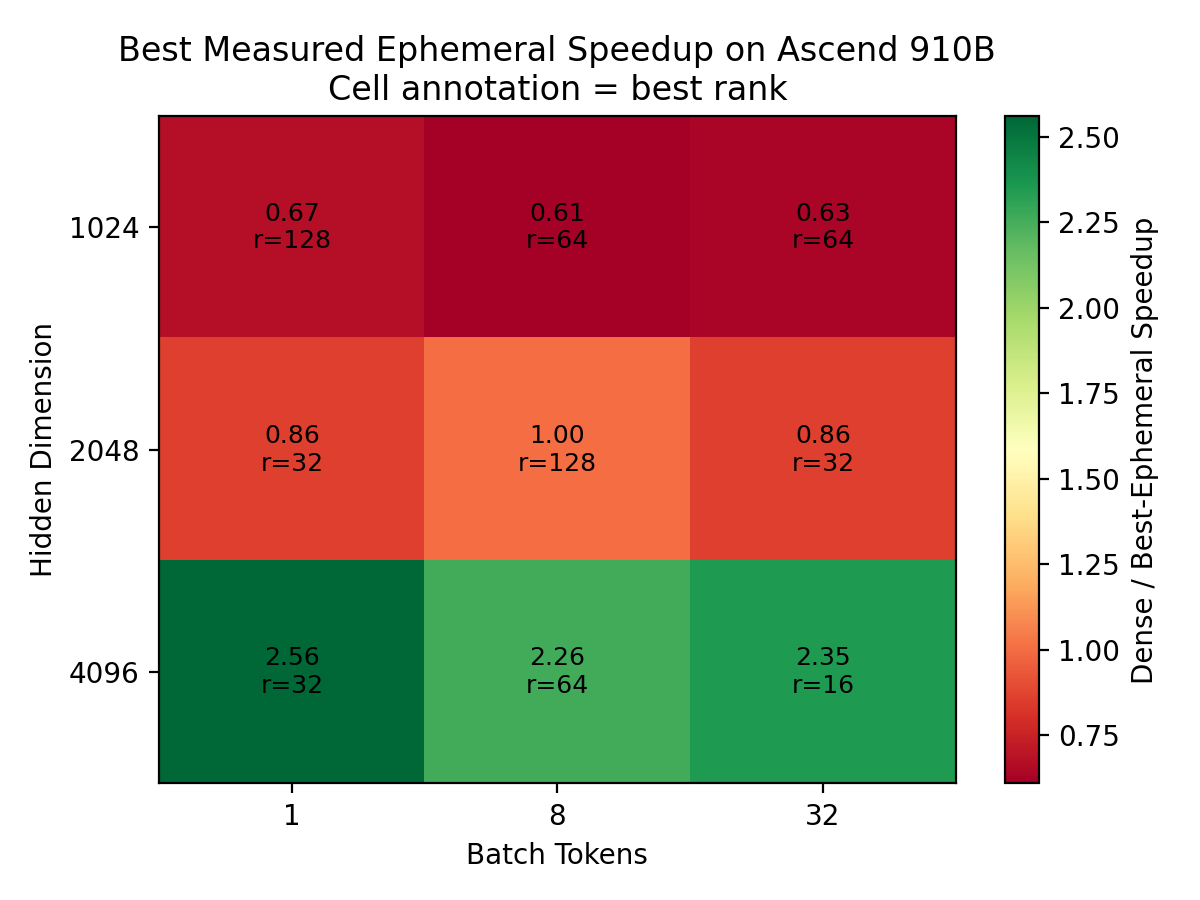
\includegraphics[width=0.72\linewidth]{figures/ai2_best_speedup_heatmap.png}
\caption{Best measured dense-to-ephemeral speedup on Ascend 910B over five independent trials per configuration. Each cell reports the best mean speedup for a $(b,d)$ bucket; the annotation shows the best-performing rank.}
\label{fig:ai2-heatmap}
\end{figure}

To sharpen the crossover boundary, we ran an additional five-trial rank sweep focused on the ambiguous regime. This sweep uses $d \in \{2048,4096\}$, $b \in \{1,8,32\}$, and ranks from $8$ to $256$ on a denser grid. The result resolves the medium-size question in favor of the dense baseline: for $d=2048$, the best measured ephemeral mean remains below parity for all three batch-token counts, with peak dense-to-ephemeral speedups of only $0.90\times$--$0.96\times$. By contrast, $d=4096$ remains robustly favorable, with best ranks between $16$ and $32$ for $b \in \{1,32\}$ and $32$ for $b=8$, achieving $2.36\times$--$2.57\times$ speedup. Figure~\ref{fig:ai2-frontier} shows that the useful region on 910B is not simply ``low rank'' in the abstract: ranks $16$--$64$ form a broad plateau, while some poorly aligned ranks such as $8$ and $24$ suffer marked latency penalties.

\begin{figure}[t]
\centering
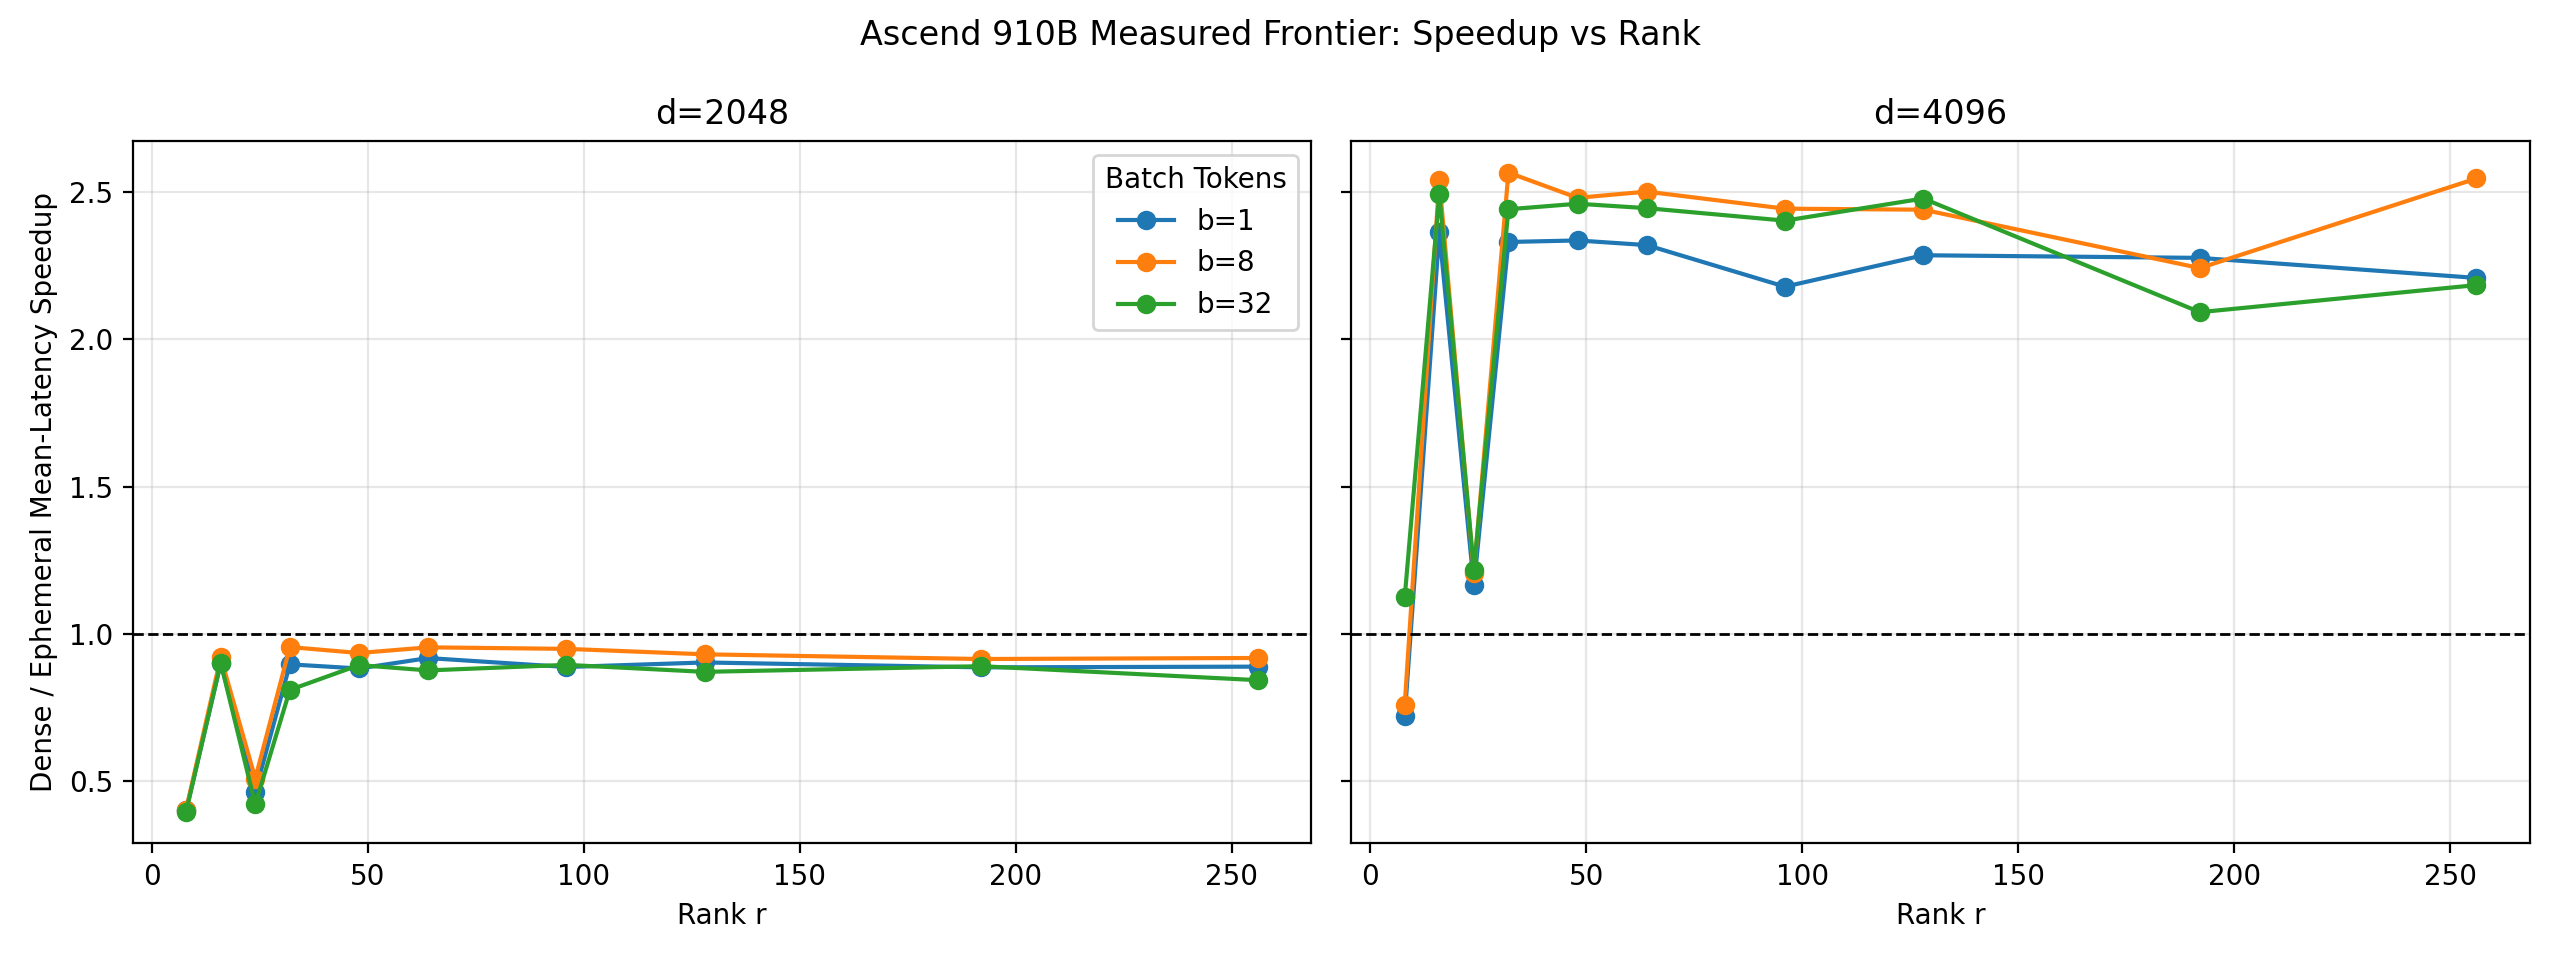
\includegraphics[width=0.95\linewidth]{figures/ai2_frontier_speedup_vs_rank.png}
\caption{Measured dense-to-ephemeral speedup versus rank on Ascend 910B for the denser five-trial frontier sweep. The $d=2048$ curves stay below the break-even line across all tested ranks, while the $d=4096$ curves remain clearly above break-even over a broad band centered around $r=16$--$64$.}
\label{fig:ai2-frontier}
\end{figure}

We next asked whether this advantage survives in settings closer to deployed transformer blocks, rather than isolated factorized linear maps. To do so, we benchmarked three application-style proxies on ai2: a full two-layer FFN block with activation, a SwiGLU-style gated FFN block, and a top-2 MoE-style expert block in which router probabilities mix two FFN experts. For each scenario we measured three variants end-to-end on the device: dense execution, a static low-rank ephemeral approximation, and a \emph{dynamic} ephemeral proxy in which token-conditioned coefficients synthesize low-rank factors from a small learned basis within the measured forward path. The application benchmark uses hidden dimensions $d \in \{2048,4096,8192\}$, batch-token counts $b \in \{1,8,32\}$ to span decode-like and short-to-medium prefill settings, ranks $r \in \{16,32,64\}$, and three independent trials per configuration.

These broader application proxies make two points more clearly. First, the \emph{static} ephemeral mechanism transfers across a wide range of block structures: it beats dense execution in $22$ of $27$ measured scenario-shape buckets. At $d=4096$, the best static ephemeral variants reach about $2.3\times$--$3.8\times$ speedup depending on the block type, and at $d=8192$ they rise to about $7.4\times$--$16.6\times$. Second, once generator cost is moved into the measured path, the useful region narrows again but does not disappear. The dynamic basis-generated proxy wins in $9$ of $27$ buckets, and all of those wins occur at $d=8192$ across FFN, SwiGLU, and MoE-style blocks, where measured speedups reach about $3.0\times$--$3.8\times$. This is a stronger and more careful formulation of the paper's thesis: dynamic generation is not broadly favorable at moderate hidden sizes under an unfused implementation, but it can still replace memory movement profitably for large transformer blocks and across multiple architectural motifs. Figure~\ref{fig:ai2-applications} summarizes these application-scenario results.

\begin{table}[t]
\centering
\begin{tabular}{@{}llll@{}}
\toprule
Evidence & Regime & Best measured speedup & Interpretation \\
\midrule
Operator microbench & $d=4096$ & $2.26\times$--$2.56\times$ & Clear crossover above dense \\
Operator microbench & $d=2048$ & $0.90\times$--$1.00\times$ & At or below parity \\
Application, static & $d=4096$ & $2.3\times$--$3.8\times$ & Transfers across block types \\
Application, static & $d=8192$ & $7.4\times$--$16.6\times$ & Strong large-shape benefit \\
Application, dynamic & $d=8192$ & $3.0\times$--$3.8\times$ & Generator-aware wins emerge \\
\bottomrule
\end{tabular}
\caption{Condensed view of the main empirical result. Static ephemeral factorization is broadly favorable once shapes are large enough, while dynamic generation only becomes favorable in the largest measured regime.}
\label{tab:main-summary}
\end{table}

\begin{figure}[t]
\centering
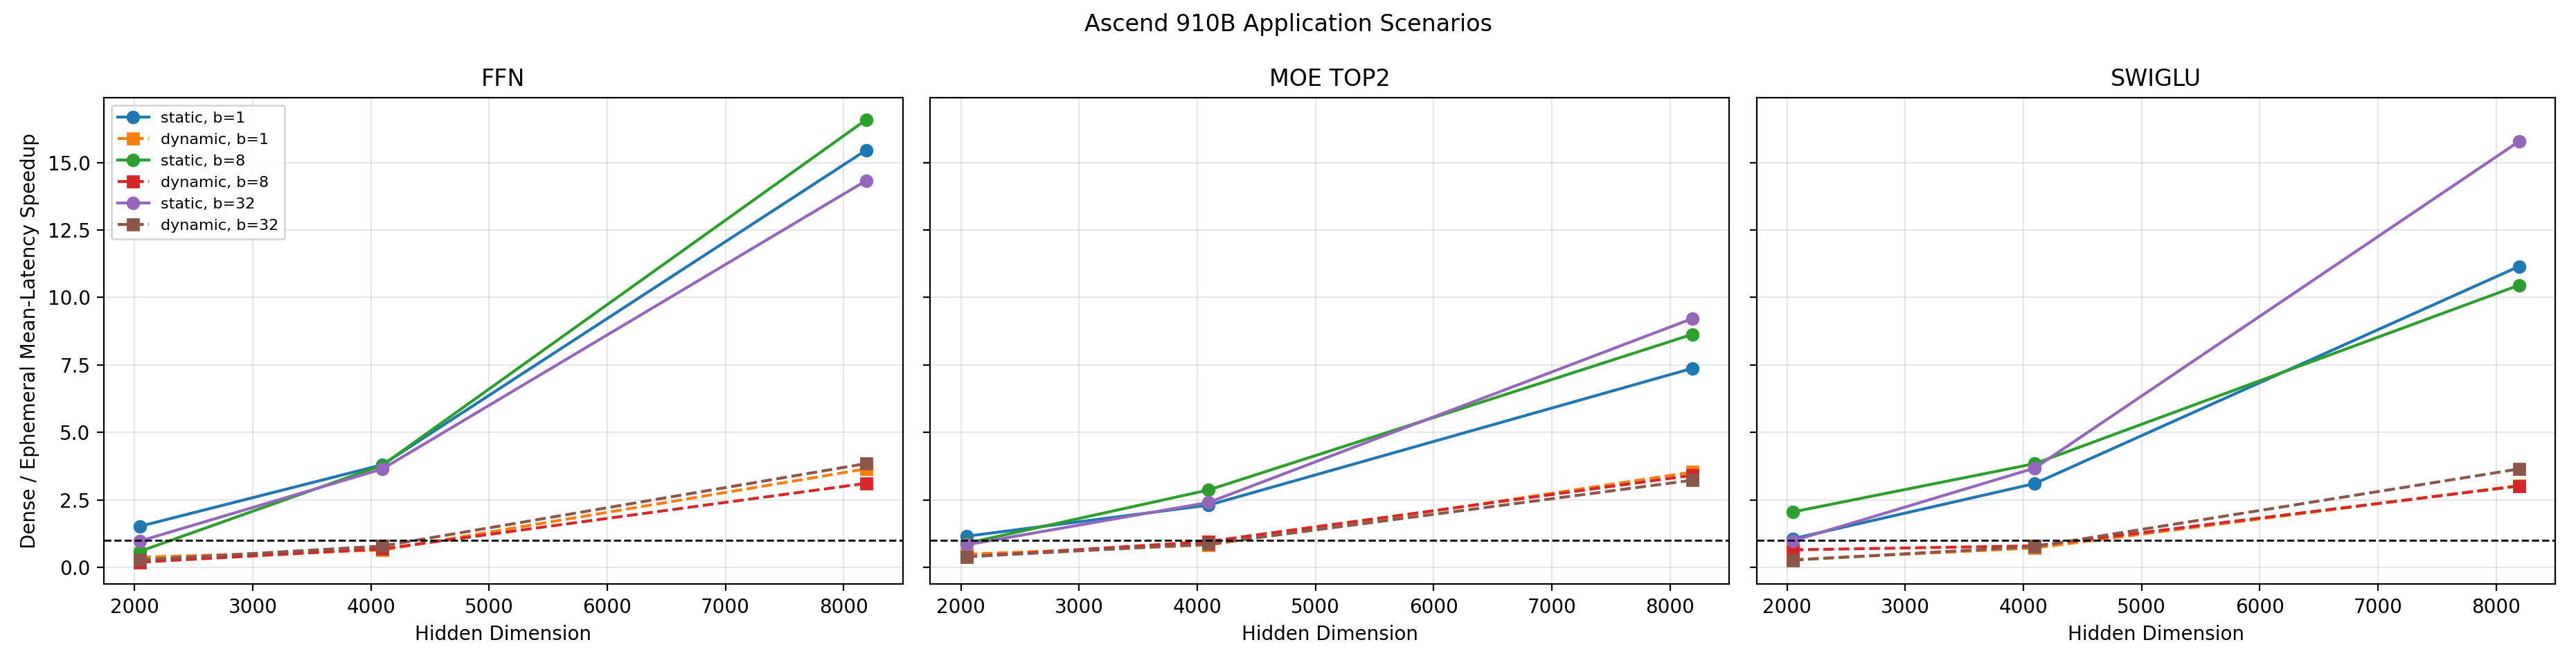
\includegraphics[width=0.95\linewidth]{figures/ai2_application_scenarios.png}
\caption{Best measured speedups for static and dynamic ephemeral execution across FFN, SwiGLU, and top-2 MoE proxies on Ascend 910B. Static factorization transfers broadly, while dynamic generation becomes favorable only at $d=8192$.}
\label{fig:ai2-applications}
\end{figure}

\subsection{Simulator--Measurement Gap}
To document the calibration problem explicitly, we compared the 910B-like simulator against the measured ai2 results. The simulator consistently overestimates the benefit of ephemeral execution, especially at small and medium sizes. In the current uncalibrated model, simulated speedups for some $d=4096$ settings exceed $200\times$, whereas the repeated measured speedups are closer to $2.26\times$--$2.56\times$. This gap indicates that the dominant missing terms are not high-level FLOP counts but systems effects such as launch overhead, imperfect fusion, operator scheduling, and achieved-versus-peak utilization.

This discrepancy improves the paper rather than weakening it: it allows us to state a sharper and more defensible claim. The correct claim is not that roofline analysis alone proves massive speedups, but that roofline analysis identifies promising memory-bound regimes, while actual 910B measurements confirm a narrower but still meaningful win region.

\section{Discussion and Limitations}
The paper supports three claims, and only three. First, roofline analysis is useful for identifying where the memory-wall hypothesis may be relevant, but on its own it materially overpredicts the achievable speedup. Second, on Ascend 910B there is a reproducible operator-level crossover for sufficiently large FFN blocks, with $d=4096$ clearly favorable and $d=2048$ not robustly favorable. Third, the broader application-style measurements show that \emph{static} ephemeral factorization transfers across several transformer block motifs, whereas \emph{dynamic} generation remains a large-shape effect under the unfused proxy implemented here.

Several limitations remain. The dynamic path in this paper is a conservative proxy rather than a fused production kernel, so the measured dynamic results should be interpreted as evidence of feasibility under explicit generator cost, not as a final upper bound on deployment performance. The experiments also focus on latency for isolated operators and block-level proxies rather than full-model quality or end-to-end serving throughput. Finally, the study targets one hardware family, Ascend 910B, and therefore should be read as a hardware-contingent systems result rather than a universal statement about all accelerators.

\section{Conclusion}
On-the-fly ephemeral weights are a systems-and-architecture hypothesis: spend extra compute to avoid expensive parameter movement. The evidence in this paper supports a narrower but more defensible version of that hypothesis than a naive roofline argument would suggest. On Ascend 910B, static factorized execution already yields large wins for sufficiently large FFN-like blocks, while dynamic generation becomes favorable only once hidden sizes are large enough for memory-traffic savings to dominate generator overhead. The resulting picture is not ``ephemeral weights always win,'' but rather that there exists a measurable large-shape regime in which replacing weight movement with additional compute is beneficial and practically relevant.

\bibliographystyle{plain}
\bibliography{references}

\end{document}
